%نام و نام خانوادگی:
%شماره دانشجویی: 
\مسئله{عبارت آرمانی}

\پاسخ{
\begin{enumerate}
	\item
	علاوه بر پارس‌استک PS 
	یک استک جدید به نام TS تعریف می‌کنیم که در هنگام پارس کردن به کمک ما می‌آید. به این صورت که هر موقع + داشتیم آن را به TS اضافه می‌کنیم و هرگاه یه - رسیدیم از استک TS POP می‌کنیم.
	 عملیات پارس به‌صورت معمول با PS انجام می‌شود و علاوه بر حالت‌های invalid که ممکن است در PS رخ دهد زمانی که باید از TS POP کنیم و TS خالی باشد نیز باید حالت invalid تشخیص داده‌شود.
		\begin{figure}[H]
			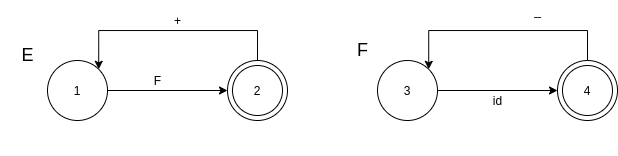
\includegraphics[width=\linewidth]{./commons/Q2part1.png}
			\label{fig:Q2}
		\end{figure}
	\item
	تنها با استفاده از گراف نحو و یک استک این کار امکان‌پذیر نیست.
\end{enumerate}
}
